% Created with jtex v.1.0.20
\documentclass{article}
\PassOptionsToPackage{short, nodayofweek}{datetime}


% Start Curvenote Definitions

% Pass Options Section
% base
\PassOptionsToPackage{normalem}{ulem}
\PassOptionsToPackage{utf8}{inputenc}

% template
\PassOptionsToPackage{framemethod=TikZ}{mdframed}
\PassOptionsToPackage{x11names, svgnames}{xcolor}

%%% PACKAGES

% base
\usepackage{inputenc}
\usepackage{url}
\usepackage{graphicx}
\usepackage{adjustbox}
\usepackage{amssymb}
\usepackage{amsfonts}
\usepackage{amsmath}
\usepackage{enumitem}
\usepackage{nicefrac}
\usepackage{booktabs}
\usepackage{microtype}
\usepackage{hyperref}
\usepackage{ulem}
\usepackage{enumitem}
\usepackage{float}
\usepackage{datetime}
\usepackage{xkeyval}
\usepackage{framed}
\usepackage{doi}

% template
\usepackage{natbib}
\usepackage{fancyvrb}
\usepackage{mdframed}
\usepackage{xcolor}

%%%


%%%% Setup Section

% base
\graphicspath{{.}}
% template
\sloppy
\newenvironment{aside}{\begin{framed}}{\end{framed}}
\newmdenv[linewidth=2pt,linecolor=CornflowerBlue,topline=false,bottomline=false,rightline=false,leftline=true,skipabove=20,skipbelow=20,leftmargin=20,rightmargin=20]{callout}
\newfloat{code}{thp}{loc}
\floatname{code}{Program}
\raggedbottom
\bibliographystyle{abbrvnat}
\setcitestyle{authoryear,open={(},close={)},semicolon,aysep={,}}

% End Curvenote Definitions


%%%%%%%%%%%%%%%%%%%%%%%%%%%%%%%%%%%%%%%%%%%%%%%%%%
%%%%%%%%%%%%%%%%%%%%  imports  %%%%%%%%%%%%%%%%%%%
\usepackage{amsthm}
%%%%%%%%%%%%%%%%%  math commands  %%%%%%%%%%%%%%%%
\newcommand{\Real}{\mathbb{R}}
\newcommand{\R}{\mathbb{R}}
\newcommand{\CH}{\mathsf{CH}}
\newcommand{\eps}{\varepsilon}
%%%%%%%%%%%%%%%%%%%%%%%%%%%%%%%%%%%%%%%%%%%%%%%%%%
%%%%%%%%%%%%%%%%%%%%%%%%%%%%%%%%%%%%%%%%%%%%%%%%%%
%%%%%%%%%%%%%%%%%%%%  theorem  %%%%%%%%%%%%%%%%%%%
\newtheorem{theorem}{Theorem}[section]
\newtheorem{corollary}{Corollary}[theorem]
\newtheorem{lemma}[theorem]{Lemma}
\newtheorem{proposition}{Proposition}[section]
\newtheorem{definition}{Definition}[section]
\newtheorem{example}{Example}[section]
\newtheorem{remark}{Remark}[section]
\newtheorem{axiom}{Axiom}[section]
\newtheorem{conjecture}{Conjecture}[section]
\newtheorem{observation}{Observation}[section]
%%%%%%%%%%%%%%%%%%%%%%%%%%%%%%%%%%%%%%%%%%%%%%%%%%




% colors for hyperlinks
\hypersetup{colorlinks=true, allcolors=blue}
\hypersetup{
pdftitle={\@title},
pdfsubject={},
pdfauthor={\@author},
pdfkeywords={},
addtopdfcreator={Written in Curvenote}
}

\usepackage{curvenote}

\title{My PDF}

\newdate{articleDate}{29}{12}{2024}
\date{\displaydate{articleDate}}

\author{}

\begin{document}

\maketitle

\begin{frame}
\frametitle{Introduction: Perfect Subsets of the Real Line}

\begin{framed}
\textbf{Continuum Hypothesis (Cantor, 1890s)}\\
If $A \subseteq \Real$ is uncountable, then there exists a bijection between $A$ and $\Real$. That is, is every uncountable subset of $\Real$ is of the same cardinality as $\Real$.
\end{framed}

Possible approach: show that $\CH$ holds for a number of sets with an easy topological structure.

\begin{framed}
\textbf{Exercise}\\
Show that every open set in $\R$ satisfies $\CH$ (in the sense that it either countable or can be mapped bijectively to $\R$).
\end{framed}

Closed sets?

Given a set $A \subseteq \Real$, we call $x \in \Real$ an \textbf{limit point} of $A$ if

\begin{equation}
\forall \epsilon > 0 \: \exists z \in A \: [z \neq x \: \& \: z \in U_\eps(x)],
\end{equation}

where $U_\eps(x)$ denotes the standard $\eps$-neighborhood of $x$ in $\Real$

A non-empty set $P \subseteq \Real$ is \textbf{perfect} if it is closed and every point of $P$ is an limit point.

In other words, a perfect set is a closed set that has no isolated points.

For a perfect set $P$, every neighborhood of a point $p \in P$ contains infinitely many points from $P$.

Obviously, $\Real$ itself is perfect, as is any closed interval in $\Real$. There are totally disconnected perfect sets, such as the \textbf{middle-third Cantor set} in $[0,1]$

\begin{figure}[!htbp]
\centering
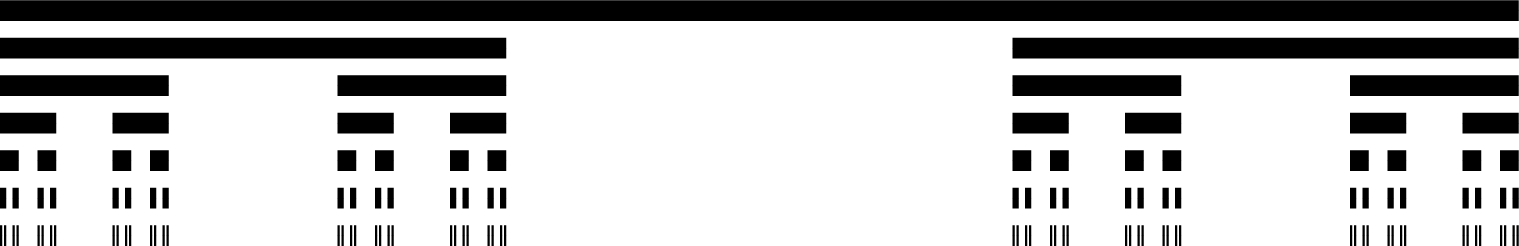
\includegraphics[width=0.7\linewidth]{files/Cantor_set-7f15a3eb647d25cf38092c5cd78d7432.png}
\end{figure}

\begin{theorem}[Cantor, 1884]\label{thm-card-perfect-sets}A perfect subset of $\Real$ has the same cardinality as $\Real$.

\end{theorem}\begin{theorem}[Cantor-Bendixson]\label{cantor-bendixson}Every uncountable closed subset of $\Real$ contains a perfect subset.

\end{theorem}\begin{corollary}Every closed subset of $\Real$ is either countable or of the cardinality of the continuum.

\end{corollary}\begin{definition}A family $\mathcal{F}$ of sets (of reals) has the \textbf{perfect set property} if every set in $\mathcal{F}$ is either countable or has a perfect subset.

\end{definition}\begin{framed}
\textbf{Question}\\
Which families of sets have the perfect set property?
\end{framed}

\end{frame}
\end{document}
